%!TEX root = ../notas_de_clase.tex

\newpage
\section{Redes Neuronales}

\subsection{Introducción y arquitectura}

\subsubsection{Conceptos básicos}

Los modelos escenciales de redes neuronales se conocen como \textbf{feedforward neural networks}, o \textbf{multilayer perceptrons} (MLPs). Una red neuronal busca aproximar una funci\'on $f^*$. Una red feedforward define un mapping $\bm{y}=f(\bm{x}; \bm{\theta})$ y aprende los par\'ametros $\bm{\theta}$ que resultan en la mejor aproximaci\'on posible.

Estos modelos se conocen como redes ya que que t\'ipicamente son el resultado de composiciones sucesivas de varios tipos de funciones. Por ejemplo, sean $f^{(1)}$, $f^{(2)}$ y $f^{(3)}$ funciones, estas se 'conectan' para formar $f(\bm{x}) = f^{(3)}(f^{(2)}(f^{(1)}(\bm{x})))$, se dice que $f^{(1)}$ es la primera \textbf{capa} de la red, $f^{(2)}$ la segunda y $f^{(3)}$ la tercera. El largo de esta cadena define la \textbf{profundidad} de la red. El uso de redes neuronales con m\'ultiples capas se conoce como \textbf{deep learning}, aunque este t\'ermino se usa para problemas m\'as espec\'ificos de aprendizaje de m\'aquinas usando redes neuronales profundas (ver secci\'on 3.5).

Durante el entrenamiento de una red neuronal se busca que $f(\bm{x}) \approx f^*(\bm{x})$, donde la data de entrenamiento provee aproximaciones ruidosas de $f^*(\bm{x})$. Cada dato $\bm{x}$ viene acompa{\~{n}}ado de una etiqueta, $y \approx f^*(\bm{x})$. Los datos de entrenamiento indica qu\'e debe reproducir la red en su \'ultima capa, lo cual debe ser un valor aproximado de $y$. El comportamiento del resto de las capas no tiene una interpretación tan directa como la última capa, por lo que el algoritmo de aprendizaje debe decidir c\'omo adaptar las capas para que el output producido por la red sea lo m\'as cercano posible a $y$, la etiqueta, para cada punto $\bm{x}$. Es por esto que estas capas intermedias se denominan \textbf{capas ocultas}.

Estas redes se llaman \textit{neuronales} por su inspiraci\'on neurocient\'ifica. Cada capa oculta de la red corresponde a un vector. Se podr\'ia pensar que cada elemento de estos vectores tiene un rol similar al de una neurona, en vez de pensar cada capa como una funci\'on que produce un mapping de vector a vector, podr\'ia considerarse que una capa consiste en muchas \textbf{unidades} que act\'uan en paralelo, cada una representando un mapping de vector a escalar. La elecci\'on de las funciones $f^{(i)}(\bm{x})$, conocidas como \textbf{funciones de activaci\'on}, en varios casos ha sido guiada por observaciones sobre el comportamiento de neuronas biol\'ogicas.

\begin{figure}[H]
\captionsetup{font=small,labelfont=small}
\caption{Ejemplo de una red neuronal de 1 capa: (\textit{izquierda}) Se muestra la red con inputs $x_1$ y $x_2$, que luego pasan a la capa oculta para producir el output $y$. (\textit{derecha}) Misma red con una representaci\'on vectorial de las capas. La matriz ${\bm{W}}$ describe el mapping de ${\bm{x}}$ a ${\bm{h}}$, y la matriz $w$ el mapping de ${\bm{h}}$ a $y$.}
\centering
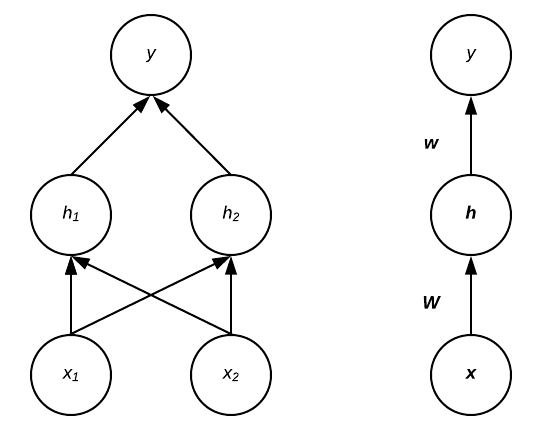
\includegraphics[scale=.5]{img/cap7_F1NN1L.png}
\end{figure}

Como se puede apreciar en la figura, los coeficientes ${\bm{W}}$ y $w$ se usan para producir el output para la siguiente capa (denominados \textbf{pesos}), por lo que la primera operaci\'on de esta red ser\'a entregar $h_{1}$ y $h_{2}$ mediante la transformaci\'on ${\bm{W}^{T}}\bm{x} + \bm{b}^{(1)}$. Luego, esta red aplica $w^{T} \boldsymbol{h} + b^{(2)}$ para producir el output $y$. Los coeficientes $\bm{b}^{(1)}$ y  $b^{(2)}$ se conocen como t\'erminos de \textbf{bias} (sesgo). Todos los parámetros de la red neuronal, los pesos y \textit{bias}, serán agrupados en el t\'ermino $\bm{\theta}$.

\subsubsection{Funci\'on de costos, unidades de output y la formulaci\'on como un problema probabil\'istico}

Una de las principales diferencias entre los modelos lineales antes vistos y una red neuronal, es que el uso de ciertas funciones de activaci\'on hacen que la funci\'on de costos no sea convexa, esto hace que el entrenamiento realizado en base a descenso de gradiente no entregue garant\'ias de que se alcanzar\'a el \'optimo global, o una buena solución en términos generales, ya que el algoritmo podría estancarse en un optimo local que entregue resultados pobres. 

En la mayor\'ia de los casos, el modelo param\'etrico define una distribuci\'on $p(y|\bm{x}; \bm{\theta})$, por lo que los par\'ametros del modelo se estimar\'an usando m\'axima verosimilitud, as\'i, se optimizar\'a la log-verosimilitud negativa, es decir, la \textbf{funci\'on de costos} a usar ser\'a la \textbf{cross-entropy}:

\begin{equation}
J(\bm{\theta}) = -\E_{\bm{x},\bm{y}\sim \hat{p}_{\textrm{data}}}(\textrm{log}\; p_{\textrm{modelo}}(\bm{y}|\bm{x}))
\end{equation}

De esta forma la elecci\'on de la \textbf{unidad de output} definir\'a la forma que toma la funci\'on de costos, pero no ser\'a necesario definir una funci\'on especifica para cada problema; en general siempre se resolver\'a el problema por m\'axima verosimilitud. La elecci\'on en la unidad de output depender\'a del tipo de problema que se quiera resolver. Cuando se quiera retornar la media de una distribuci\'on Gaussiana condicional, $p(\bm{y}|\bm{x}) = \mathcal{N}(\bm{y}|\hat{\bm{y}};\bm{I})$, la unidad de output deber\'a ser un modelo lineal, $\hat{\bm{y}} = \bm{W}^{T}\bm{h} + \bm{b}$, en donde $\bm{h}$ es el output de la red que proviene de todas las capas ocultas anteriores. En este caso, maximizar la log-verosimilitud es equivalente a minimizar el error cuadr\'atico medio, por esta razón este tipo de output es adecuada para un problema de regresión.

Cuando el problema objetivo es clasificaci\'on binaria, una unidad de output apropiada es la funci\'on sigmoidal. Para resolver el problema de m\'axima verosimilitud, se modela utilizando una distribuci\'on Bernoulli en $y$ condicional en $\bm{x}$. Una unidad de output sigmoidal se define como $\hat{{y}} = \sigma(\bm{w}^{T}\bm{h} + {b})$. Esto entrega como output $P(y=1|\bm{x})$, por lo que se podr\'a decidir a qu\'e clase pertenece $y$ basado en el output de la red, esto se interpreta como la probabilidad de que la observaci\'on sea de la clase 1.

Para un problema de clasificaci\'on multiclase, la unidad de output apropiada es la generalizaci\'on de la funci\'on sigmoidal, conocida como softmax. El problema es predecir a cu\'al de $n$ clases pertenece $y$, por lo que se requiere producir un vector $\hat{\bm{y}}$, con $\hat{y_{i}} = P(y=i|\bm{x})$, por lo que se usar\'a una distribuci\'on multinoulli. Primero, una capa lineal predice las log-probabilidades no normalizadas, $\bm{z} = \bm{W}^{T}\bm{h} + \bm{b}$, y luego se aplica la funci\'on softmax para obtener los valores de $\hat{\bm{y}}$ antes descritos:

\begin{equation}
\textrm{log softmax}(\bm{z})_{i} = \textrm{log}\frac{\textrm{exp}(z_{i})}{\sum_{j=1}^{n}\textrm{exp}({z_{j}})} = z_{i} - \textrm{log}\sum_{j=1}^{n}\textrm{exp}({z_{j}})
\end{equation}

\subsubsection{Estructura interna de la red}

Las capas escondidas proveen a la red neuronal la flexibilidad necesaria para aprender funciones extremadamente complejas, esto mediante el uso de activaciones no lineales. En varios casos estas funciones son incluso no diferenciables, lo que llevar\'ia a pensar de que no son v\'alidas para ser usadas en conjunto con algoritmos que usan descenso de gradiente, pero en la pr\'actica tienen un desempe\~{n}o suficientemente bueno para ser usadas en tareas de aprendizaje de m\'aquinas. En general, las funciones de activaci\'on para las unidades escondidas toman como input un vector $\bm{x}$ para el cual obtienen una transformaci\'on af\'in $\bm{z} = \bm{W}^{T}\bm{x} + \bm{b}$, para luego aplicar una transformaci\'on no lineal $g(\bm{z})$. Las unidades escondidas m\'as comunes son las \textbf{rectified linear units} o \textbf{ReLUs}, $g(\bm{z}) = \textrm{max}(0, \bm{z})$, y sus generalizaciones como \textbf{leaky ReLU}, $g(\bm{z})_{i} = \textrm{max}(0, \bm{z}_{i}) + \alpha_{i}\textrm{min}(0, \bm{z}_{i})$, con $\alpha_{i}$ una constante peque\~{n}a como 0.01; la funci\'on sigmoidal $g(\bm{z}) = \sigma(\bm{z})$; y la tangente hiperb\'olica $g(\bm{z}) =  \textrm{tanh}(\bm{z}) = 2\sigma(2\bm{z}) - 1$. A diferencia de las funciones lineales por partes, las unidades sigmoidales se saturan en la mayor parte de su dominio (su gradiente se aproxima a 0) haciendo imposible el aprendizaje por el gradiente cuando esto ocurre, por lo que su uso como unidades escondidas ha sido desalentado.

\subsubsection{Dise\~{n}o de arquitectura y teorema de aproximaci\'on universal}

La \textbf{arquitectura} de una red neuronal se refiere a la totalidad de su estructura: la cantidad de capas, la cantidad de unidades escondidas, la conexi\'on entre las unidades, etc. Bajo la estructura mostrada para una red feedforward, la primera capa y la segunda capa son de la forma:

\begin{equation}
\begin{split}
\bm{h}^{(1)} = g^{(1)}(\bm{W}^{(1) T}\bm{x} + \bm{b}^{(1)}) \\
\bm{h}^{(2)} = g^{(1)}(\bm{W}^{(2) T}\bm{h}^{(1)} + \bm{b}^{(2)})
\end{split}
\end{equation}

En una arquitectura de este tipo, la principal consideraci\'on respecto al dise\~{n}o es la profundidad y ancho (cantidad de unidades por capa) de cada capa. Una red con solo 1 capa escondida puede ser suficiente para ajustar el set de entrenamiento, cabe destacar que la cantidad de neuronas necesarias en esta única capa podría ser muy grande y la capacidad de generalización puede ser baja, dependiendo de la complejidad de los datos con los que se pretende trabajar. Redes m\'as profundas generalmente permiten disminuir el n\'umero de unidades por capa (de esta forma tener una menor cantidad par\'ametros en total), como as\'i tambi\'en una mejor capacidad de generalización en el set de testeo, con esto se hace referencia a la capacidad de la red para clasificar correctamente ejemplos que no fueron usados para el proceso de entrenamiento, naturalmente hacer más intrincado el diseño de la red hará que el proceso de optimización para ajustar los parámetros sea más costoso. La arquitectura ideal se debe encontrar por experimentaci\'on con distintas estructuras acompañado de conocimiento sobre el tipo de datos, esto se apoya mediante el monitoreo del error en el set de validaci\'on.

Una de las principales justificaciones para usar redes neuronales se debe al \textbf{Teorema de Aproximaci\'on Universal} (Horniket al., 1989; Cybenko, 1989), el cual muestra que una red feedforward con una capa de output lineal y al menos una capa escondida con funci\'on de activaci\'on sigmoidal (y otras similares) puede aproximar cualquier funci\'on Borel medible \footnote{En particular cualquier funci\'on continua en un subconjunto cerrado y acotado de $\R^{n}$ es Borel medible, la clase de funciones Borel medibles es mucho más rica y variada que las funciones continuas.} de un espacio dimensión finita a otro, con un nivel de error arbitrariamente pequeño, provisto de que hayan suficientes unidades escondidas. Una red neuronal tambi\'en puede aproximar un mapping de cualquier espacio dimensional finito y discreto a otro, y este teorema tambi\'en se ha probado para una amplia gama de funciones de activaci\'on, como para la m\'as com\'unmente usada ReLU (Leshno et al., 1993). La desventaja del teorema es que a pesar que asegura que la red podr\'a aproximar cualquiera de estas funciones, esto no implica que necesariamente podr\'a \textit{aprender} la funci\'on en sí. Una razón posible es que el algoritmo de optimizaci\'on podr\'ia no encontrar los par\'ametros de la red que alcancen el nivel de error deseado. Tampoco especifica la cantidad de unidades que son necesarias para alcanzar un nivel de error dado, lo cual podr\'ia ser excesivamente grande. Sin embargo en muchos casos modelos m\'as profundos necesitar\'an menos unidades y potencialmente permiten reducir el error de generalizaci\'on.

\subsection{Entrenamiento de una red neuronal}

\subsubsection{Forward propagation y back-propagation}

Al usar una red neuronal feedforward, la informaci\'on fluye a trav\'es de la red desde el ingreso de un input $\bm{x}$ hasta producir un output $\hat{\bm{y}}$. Esto se conoce como \textbf{forward propagation}. Durante el entrenamiento, \textit{forward propagation} contin\'ua hasta producir el costo escalar $J(\bm{\theta})$.

El algoritmo de \textbf{back-propagation} permite que la informaci\'on del costo fluya en sentido inverso a trav\'es de la red para calcular el gradiente de manera computacionalmente eficiente. El gradiente se calculará de esta forma ya que, aunque es posible obtener una expresi\'on anal\'itica para este, evaluar la expresi\'on puede ser muy caro computacionalmente. Luego de obtener el gradiente, otro algoritmo como descenso de gradiente estoc\'astico (ver secci\'on 4) realiza el aprendizaje usando la expresión que fue calculada. En algoritmos de aprendizaje el gradiente que m\'as com\'unmente se requiere obtener es $\nabla_{\bm{\theta}}J(\bm{\theta})$, aunque el algoritmo de \textit{back-propagation} no se limita a esto y puede ser usando para otras tareas que involucren obtener derivadas.

Sea $\bm{x} \in \R^{m}, \bm{y} \in \R^{n}, g:\R^{m} \rightarrow \R^{n}, f:\R^{n} \rightarrow \R, \bm{y} = g(\bm{x})$ y $z = f(\bm{y})$, la regla de la cadena indica que:

\begin{equation}
\frac{\partial z}{\partial x_{i}} = \sum_{j}\frac{\partial z}{\partial y_{j}}\frac{\partial y_{j}}{\partial x_{i}}
\end{equation}

O de manera equivalente visto en su forma vectorial:

\begin{equation}
\nabla_{\bm{x}}z = (\frac{\partial \bm{y}}{\partial \bm{x}})^{T}\nabla_{\bm{y}}z
\end{equation}

en donde $\frac{\partial \bm{y}}{\partial \bm{x}}$ es la matriz Jacobiana de $g$, con esto se puede ver que para obtener el gradiente con respecto a la variable $\bm{x}$, basta multiplicar la matriz Jacobiana por el gradiente con respecto a $\bm{y}$.% El algoritmo de \textit{back-propagation} consiste en realizar este tipo de operaciones iterativamente, calculando la regla de la cadena con un orden espec\'ifico de operaciones que lo hace altamente eficiente.


Usualmente se aplicar\'a \textit{back-propagation} a \textbf{tensores} de dimensionalidad arbitraria, no solo vectores. Se denota entonces el gradiente de $z$ con respecto a un tensor $\textrm{\textbf{X}}$ como $\nabla_{\textrm{\textbf{X}}}z$. Sean $\textrm{\textbf{Y}} = g(\textrm{\textbf{X}})$ y $z = f(\textrm{\textbf{Y}})$, entonces la regla de la cadena se escribe como:

\begin{equation}
\nabla_{\textrm{\textbf{X}}}z = \sum_{j}(\nabla_{\textrm{\textbf{X}}}\textrm{Y}_{j})\frac{\partial z}{\partial \textrm{Y}_{j}}
\end{equation}

%\newpage
%[AGREGAR DESCRIPCIÓN DE BACK-PROPAGATION]

Antes de proseguir a revisar los algoritmos de \textit{forward-propagation} y \textit{back-propagation} se realizará una breve deducción de \textit{back-propagation} que permitirá comprender de mejor manera el proceso de entrenamiento en una red neuronal, en primer lugar de analizará una red neuronal con solo una capa escondida, luego veremos que esto puede ser extendido de forma fácil a arquitecturas más complejas (osea, más capas).

Sea $\{ (x_i,y_i) \}_{i=1}^N$ un conjunto de puntos sobre los que se quiere ajustar los pesos de una red neuronal, el conjunto de entrenamiento es tal que  $x_i \in \R^p, y_i \in \R^K \quad \forall i=1,...,N$, el problema planteado corresponde a uno de clasificación sobre $K$ clases distintas. Adicionalmente se tiene que el error (función de perdida) puede ser escrito como:

\begin{equation}
J(\theta) = \sum_{i=1}^N J_i = \sum_{i=1}^N L(y_i, f(x_i;\theta))
\end{equation}

Donde $J_i$ corresponde a la discrepancia entre $y_i$ y el valor entregado por la red $f(x_i;\theta)$ evaluado por la función de perdida $L$. Para fijar ideas, la arquitectura de la red está compuesta por $p$ unidades de entrada, la capa escondida tiene $M$ neuronas con funciones de activación sigmoides ($\sigma(x)=\frac{1}{1-e^{-t}}$) y la capa de salida (output) tendrá $K$ unidades y una función de salida $g$. De esta forma el problema puede ser planteado como:

\begin{align}
	Z_m &= \sigma(\alpha_{0m} + \alpha_{m}^TX), \quad \forall m=1,...,M\\
	N_k &= \beta_{0k} + \beta_k^TZ, \quad\quad\quad \forall k=1,...,K\\
	O_k &= g_k(N), \quad\quad\quad\quad \forall k=1,...,K\\
	f(X) &= O\\
\end{align}

Donde $Z=(Z_1,...,Z_M)$, $N=(N_1,...,N_K)$, $O=(O_1,...,O_K)$ y se puede ver que $g:\R^K \rightarrow \R^K$, de esta forma los parámetros $\theta$ del modelo son:

\begin{align}
\{\alpha_{0m}, \alpha_m; \quad m &= 1,...,M \} \quad M(p+1) \quad \text{pesos}\\
\{\beta_{0k}, \beta_k; \quad k &= 1,...,K \} \quad K(M+1) \quad \text{pesos}\\
\end{align}

De ahora en adelante $J\equiv J(\theta)$, también es importante distinguir que es distinto calcular la derivada de $J$ respecto a un peso que está en la capa de salida y un peso que pertenece a una capa escondida, siendo el primer caso mucho más fácil de calcular, esto se justifica por el hecho que los valores de la capa de salida participan directamente en el calculo del error $J$, mientras que los valores de las neuronas escondidas no, esto se hará evidente en los cálculos. Como último preámbulo se definen las siguientes variables que nos ayudaran a hacer los cálculos más claros:

\begin{align}
z_{mi} &= \sigma(\alpha_{0m} + \alpha_{m}^Tx_i)\\
z_i &= (z_{1i},...,z_{Mi})\\
n_{ki} &= \beta_{0k} + \beta_k^Tz_i\\
n_i &= (n_{1i},...,n_{Ki})\\
o_{i} &= g(n_i)\\
o_{ki} &= (o_i)_k\\
\end{align}

Considerando que derivar es una operación lineal calcularemos la derivada de $J_i$, a partir de este termino podemos obtener la derivada de $J$ sumando sobre todo $i=1,...,N$.

\begin{align}
\frac{\partial J_i}{\partial \beta_{km}}&=
\frac{\partial J_i}{\partial o_{ki}}
\frac{\partial o_{ki}}{\partial n_{ki}}
\frac{\partial n_{ki}}{\partial \beta_{km}}\\
&= \frac{\partial J_i}{\partial o_{ki}}
g'_k(n_{ki})z_{mi}
\label{BP_beta}
\end{align}

Dado que $o_{ki}$ pertenece a la capa de salida, esto implica que participa directamente en la expresión de $J_i$ y por lo tanto la derivada $\frac{\partial J_i}{\partial o_{ki}}$ puede ser calculada directamente. El calculo recién hecho se conoce como regla delta ('delta rule') y es el paso principal de \textit{back-propagation}, este consiste en usar la regla de la cadena 2 veces sucesivamente.

Como se mencionó con anterioridad calcular la derivada de $J_i$ respecto a un peso perteneciente a una capa escondida es más engorroso, ya que las neuronas en las capas intermedias no participan directamente en el error, aún así es posible y el calculo entrega una formula recursiva que permite llegar a una expresión cerrada y explicita.

\begin{align}
\frac{\partial J_i}{\partial \alpha_{ml}}&=
\frac{\partial J_i}{\partial z_{mi}}
\frac{\partial z_{mi}}{\partial \alpha_{ml}}\\
&= \left [ \sum_{k=1}^K
\frac{\partial J_i}{\partial o_{ki}}
\frac{\partial o_{ki}}{\partial n_{ki}}
\frac{\partial n_{ki}}{\partial z_{mi}}
\right ]
\frac{\partial z_{mi}}{\partial \alpha_{ml}}\\
&= \left [ \sum_{k=1}^K
\frac{\partial J_i}{\partial o_{ki}}
\frac{\partial o_{ki}}{\partial n_{ki}}
\frac{\partial n_{ki}}{\partial z_{mi}}
\right ]\sigma'(\alpha_0+\alpha_mx_i)x_{il}\\
&= \left [ \sum_{k=1}^K
\frac{\partial J_i}{\partial o_{ki}}
g'(n_{ki})
\beta_{km}
\right ]\sigma'(\alpha_0+\alpha_mx_i)x_{il}\\
&=  \sum_{k=1}^K
\frac{\partial J_i}{\partial o_{ki}}
g'(n_{ki})
\beta_{km}
\sigma'(\alpha_0+\alpha_mx_i)x_{il}
\label{BP_alfa}
\end{align}

Al llegar a la expresión final se puede ver que todos los términos pueden ser calculados de forma explicita, en este punto se puede apreciar porqué el nombre \textit{back-propagation}, a partir de los cálculos obtenidos en las capas exteriores se pueden obtener derivadas de los pesos en capas anteriores, en este sentido la información se propaga 'hacia atrás' en la red. Finalmente reescribimos (\ref{BP_beta}) y (\ref{BP_alfa}) como:

\begin{equation}
	\frac{\partial J_i}{\partial \beta_{km}} = \delta_{ki}z_{mi}
	\quad\quad
	\frac{\partial J_i}{\partial \alpha_{ml}} = s_{mi}x_{il}
\end{equation}

Donde:

\begin{align}
\delta_{ki} &= 
\frac{\partial J_i}{\partial o_{ki}}
g'_k(n_{ki})\\
s_{mi} &= 
\sigma'(\alpha_0+\alpha_mx_i)\sum_{k=1}^K\beta_{km}\delta_{ki}
\end{align}

Las cantidades $\delta_{ki}$ y $s_{mi}$ son errores del modelo en la capa de salida y capas escondidas respectivamente, las 4 ultimas ecuaciones presentadas son conocidas como como ecuaciones de \textit{back-propagation}. Para extender el desarrollo a una red neuronal con más capas es importante notar que a partir de la capa final y la anterior se logró calcular todas las derivadas del gradiente del error, si se considerará la capa de entrada (input) como otra capa escondida más, se pueden repetir los mismos razonamientos y extenderlos a un nivel de profundidad arbitrario. 

%\newpage
A continuaci\'on se presentan los algoritmos de \textit{forward propagation} y \textit{back-propagation} para una red MLP en donde se conectan todas las unidades de una capa con la siguiente (fully connected MLP).

\begin{algorithm}[H] % H = forzar está posición 
\caption{Forward Propagation}\label{ML:Algorithm1}
\textbf{Requerir}: Profundidad de la red, $l$ \\
\textbf{Requerir}: $\bm{W}^{(i)}, i \in \{1,...,l\}$, pesos de la red \\
\textbf{Requerir}: $\bm{b}^{(i)}, i \in \{1,...,l\}$, parámetros bias de la red \\
\textbf{Requerir}: $\bm{x}$, el input \\
\textbf{Requerir}: $\bm{y}$, el output target \\
$\;\;\bm{h}^{(0)} = \bm{x}$\\
$\;\; \textrm{for} \;k = 1,...,l$:\\
$\;\;\;\;\;\;\bm{a}^{(k)} = \bm{b}^{(k)} + \bm{W}^{(k)}\bm{h}^{(k-1)}$\\
$\;\;\;\;\;\;\bm{h}^{(k)} = f(\bm{a}^{(k)})$\\
$\;\;\bm{\hat{y}} = \bm{h}^{(l)}$\\
$\;\;J = L(\bm{\hat{y}},\bm{y})$
\end{algorithm}

\begin{algorithm}[H] % H = forzar está posición
\caption{Back-Propagation}\label{ML:Algorithm2}
Luego de completar forward propagation: \\
$\bm{g} \leftarrow \nabla_{\bm{\hat{y}}} J = \nabla_{\bm{\hat{y}}} L(\bm{\hat{y}},\bm{y})$\\
$\textrm{for} \;k = l,l-1,...,1:$\\
$\;\;\;\;\nabla_{\bm{a}^{(k)}} J = \bm{g}\odot f'(\bm{a}^{(k)})$\\
$\;\;\;\;\nabla_{\bm{b}^{(k)}} J = \bm{g}$\\
$\;\;\;\;\nabla_{\bm{W}^{(k)}} J = \bm{g}\bm{h}^{(k-1)T}$\\
$\;\;\;\;\bm{g} \leftarrow \nabla_{\bm{h}^{(k-1)}} J = \bm{W}^{(k)T}\bm{g}$
\end{algorithm}

Con este algoritmo se obtienen los gradientes con respecto a todos los par\'ametros hasta la primera capa, propagando el gradiente desde una capa a la anterior mediante la \'ultima actualizaci\'on del algoritmo para cada iteraci\'on.

\subsection{Regularización para una red neuronal}

Las redes neuronales y algoritmos de deep learning son aplicados a tareas extremadamente complejas como lo son el procesamiento de im\'agenes, audio, y texto. Controlar la complejidad de un modelo no solo se reduce a encontrar el tamaño y cantidad de parámetros adecuados, como se ha visto para otros modelos de aprendizaje de m\'aquinas, sino que en la pr\'actica el modelo con el mejor ajuste por lo general ser\'a un modelo grande (profundo) que ha sido regularizado apropiadamente.%El rol que juega la regularizaci\'on en un escenario como este no es solo controlar la complejidad del modelo buscando un modelo con tama{\~{n}}o  adecuado con el correcto n\'umero de par\'ametros, como se ha visto para otros modelos de aprendizaje de m\'aquinas, si no que en la pr\'actica el modelo con el mejor ajuste ser\'a un modelo grande (profundo) que ha sido regularizado apropiadamente.

\subsubsection{Regularización ${L}^{2}$}

Una regularizaci\'on que se basa en limitar la norma de los parámetros del modelo es la ya conocida \textbf{regularizaci\'on} $\bm{L}^{2}$ (o \textbf{ridge regression}), mediante la cual se obtiene la funci\'on objetivo regularizada $\tilde{J}$:

\begin{equation}
\tilde{J}(\bm{\theta};\bm{X},\bm{y}) = J(\bm{\theta};\bm{X},\bm{y}) + \frac{\alpha}{2}||\bm{\theta}||^{2}_{2}
\end{equation}

en donde el hiperpar\'ametro $\alpha \in [0,\infty[\ $ indica que tanta importancia se le da al termino de regularización sobre el objetivo, no habrá regularizaci\'on cuando $\alpha = 0$ y se observará un mayor efecto regularizador a medida que $\alpha$ crece. Cabe destacar que t\'ipicamente en una regularizaci\'on por la norma solo se regularizan los \textit{pesos}, dejando los t\'erminos de \textit{bias} sin regularizar. Esto ya que cada t\'ermino de \textit{bias} controla el comportamiento de solo 1 variable implicando que no se introduce mucha varianza \textbf{[(\textit{overfitting}), no se si es pertinente esta acotación]*} al dejarlos sin regularizar, por otro lado regularizar los \textit{bias} puede inducir un alto nivel de \textit{underfitting}.

\subsubsection{Dropout}

\textbf{Bagging} consiste en entrenar m\'ultiples modelos y evaluarlos en cada dato del set de testeo. Esto no es pr\'actico para redes neuronales\textbf{[Duda, según lo que vi baggin se refiera a cuando se entrenan muchos clasificadores y luego votan sobre el resultado]*}, ya que un solo modelo puede ser muy caro de entrenar y evaluar. \textbf{Dropout} provee una aproximaci\'on barata (computacionalmente) para entrenar y evaluar \textit{bagged} ensambles compuestos por una cantidad exponencial de redes neuronales. Dropout entrena los ensambles de posiblemente todas las subredes que se puedan formar al remover unidades (que no sean las de output) de un modelo de red neuronal (ver figura). Esto se puede realizar al multiplicar por 0 el output de alguna unidad para la mayor\'ia de los casos. Espec\'ificamente, para entrenar con dropout se usa un algoritmo por mini-batches (ver secci\'on 4) para que en cada iteraci\'on se entrene una subred aplicando una m\'ascara binaria a todas las capas de input y escondidas. Los hiperpar\'ametros de este m\'etodo de regularizaci\'on corresponden al dise{\~{n}}o de la m\'ascara binaria, especificando la probabilidad de que se incluya una unidad de input y la probabilidad de que se incluya una unidad escondida. T\'ipicamente se usan los valores 0.8 y 0.5, respectivamente, sin embargo estos deben ser ajustados para controlar el nivel de regularizaci\'on (mayor valor para las probabilidades implica menor efecto regularizador) para obtener un desempe{\~{n}}o \'optimo en el set de validaci\'on.

\begin{figure}[H]
\captionsetup{font=small,labelfont=small}
\caption{Dropout entrena potencialemente todas las subredes que se puedan formar a partir de la red neuronal original (primer recuadro) al apagar el output que producen las distintas unidades}
\centering
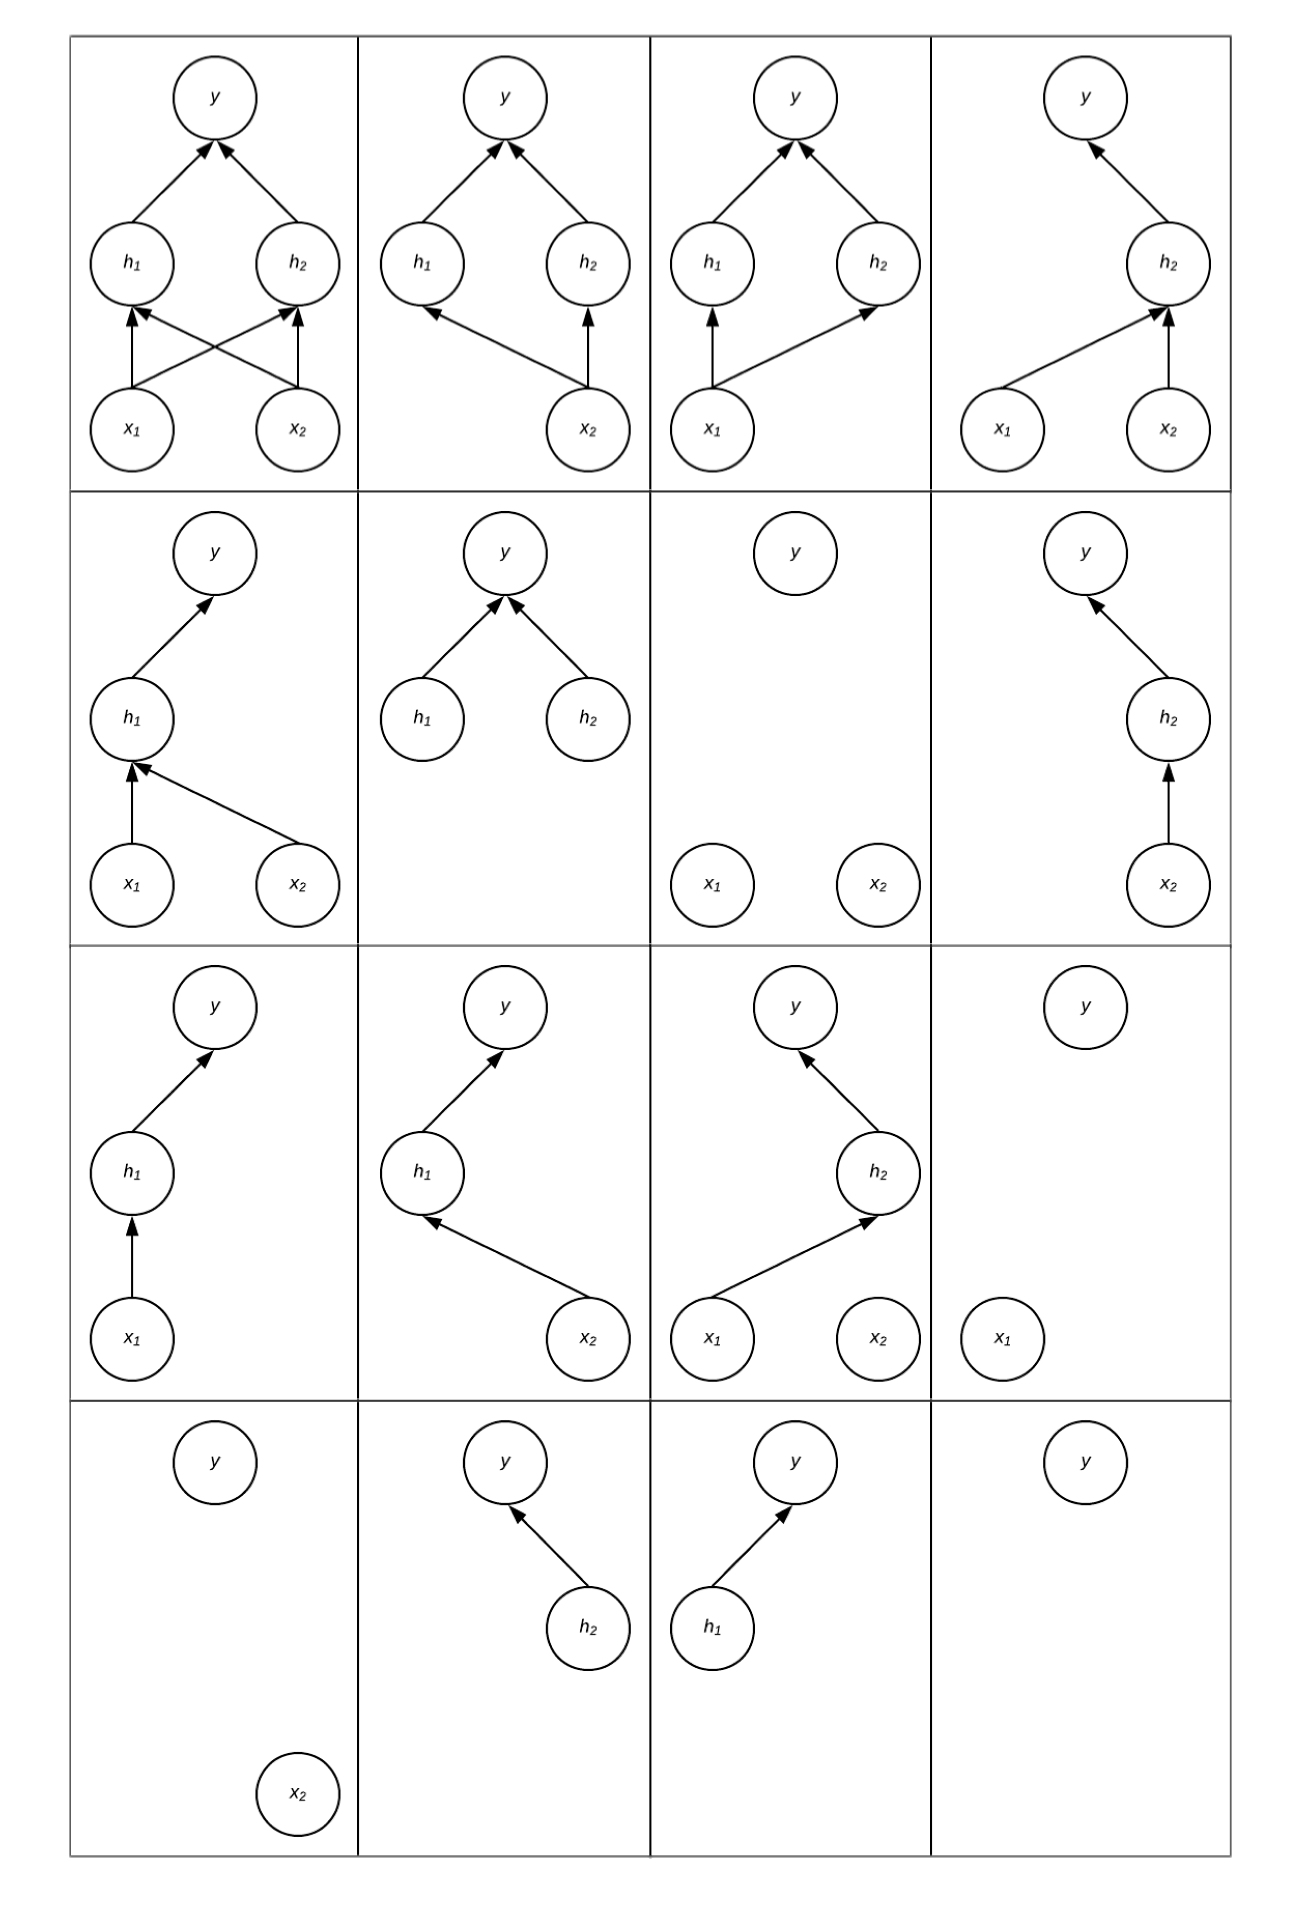
\includegraphics[scale=.25]{img/cap7_Dropout.png}
\end{figure}

\subsubsection{Otros m\'etodos de regularizaci\'on}
Otras formas de regularizaci\'on tambi\'en buscan introducir alguna fuente de ruido (como en dropout) para que la red neuronal aprenda principalmente los par\'ametros m\'as importantes, as\'i logrando un bajo error de generalizaci\'on. Una de estas t\'ecnicas es \textbf{dataset augmentation}, que consiste en generar nuevos datos de entrenamiento (inyectando ruido en el set de entrenamiento), creando datos $\bm{x}$ falsos para los cuales se pueda tener una etiqueta $y$ (por ejemplo, una imagen invertida de un gato sigue siendo un gato), o \textbf{entrenamiento adversarial}, en donde se perturban ejemplos para fortalecer a la red (por ejemplo, cambiar pixeles de una imagen que generen cambios imperceptibles para un humano pero que pueden afectar fuertemente la capacidad de predicci\'on de un modelo). Otra t\'ecnica es \textbf{noise injection} en los pesos (Jim et al., 1996; Graves, 2011), lo cual se puede interpretar como una implementaci\'on estoc\'astica de inferencia Bayesiana sobre los pesos, debido a que el aprendizaje considerar\'ia que los pesos son inciertos y, por lo tanto, representables mediante una distribuci\'on de probabilidad.

Tambi\'en, por supuesto, \textbf{early stopping} es una t\'ecnica v\'alida para regularizar redes neuronales.

\subsection{Algoritmos de optimizaci\'on}

Como ya se ha comentado, la optimizaci\'on en redes neuronales busca resolver un problema particular: encontrar los par\'ametros $\bm{\theta}$ que disminuyan significativamente $J(\bm{\theta})$, que depende de alguna medida de desempe{\~{n}}o evaluada en la totalidad del set de entrenamiento, luego se evaluá el error en el set de validaci\'on para tener una idea del desempeño, finalmente se ven los resultados en el set de testeo. 

Esto se reduce a minimizar la esperanza del error sobre la distribuci\'on generadora de los datos, $p_{\textrm{data}}$:

%[ posiblemente minimizando mediante hiperpar\'ametros tambi\'en una funci\'on de costos regularizada $\tilde{J}(\bm{\theta})$ ]

\begin{equation}
J^{*}(\bm{\theta}) = \E_{(\bm{x},y)\sim {p}_{\textrm{data}}}L(f(\bm{x};\bm{\theta}),y)
\label{gradiente_completo}
\end{equation}

Reemplazamos la expresión anterior por un problema sustituto, que consiste en escribir la funci\'on de costos como un promedio sobre el set de entrenamiento, como se puede observar la diferencia entre las dos expresiones radica en el hecho que se considera que los datos fueron generados por distribuciones de probabilidad distintas (${p}_{\textrm{data}}$ en la primera expresión, $\hat{p}_{\textrm{data}}$ en la segunda):

\begin{equation}
J(\bm{\theta}) = \E_{(\bm{x},y)\sim \hat{p}_{\textrm{data}}}L(f(\bm{x};\bm{\theta}),y) = \frac{1}{m}\sum_{i=1}^m L(f(x^{(i)};\theta),y^{(i)})
\end{equation}

\subsubsection{Minibatch}

Los algoritmos de optimizaci\'on para aprendizaje de m\'aquinas t\'ipicamente actualizan los par\'ametros usando un valor esperado del costo, obtenido a trav\'es de un subset de los t\'erminos de la funci\'on de costos. La propiedad m\'as usada respecto de la funci\'on objetivo (1) es sobre el gradiente, este cumple la siguiente expresión:

\begin{equation}
\nabla_{\bm{\theta}}J(\bm{\theta}) = -\E_{\bm{x},y\sim \hat{p}_{\textrm{data}}}\nabla_{\bm{\theta}}\textrm{log}\; p_{\textrm{modelo}}(y|\bm{x})
\end{equation}

Calcular esta expresi\'on es computacionalmente caro, ya que requiere evaluar cada ejemplo del set de entrenamiento, por lo que se puede optar por samplear un peque{\~{n}}o n\'umero de ejemplos para obtener este valor esperado, calculando el promedio usando solo estos ejemplos. Los algoritmos de optimizaci\'on que usan el set de entrenamiento completo para actualizar los par\'ametros en cada iteraci\'on se conocen como \textbf{m\'etodos de batch} o \textbf{determin\'isticos}. Los algoritmos que usan un solo ejemplo a la vez se conocen como \textbf{m\'etodos estoc\'asticos} u \textbf{online} (aunque el t\'ermino \textit{online} se suele usar para describir un entrenamiento con un flujo continuo de nuevos ejemplos). La mayor\'ia de los algoritmos usados pertenecen a una categor\'ia intermedia, estos son los \textbf{m\'etodos de minibatch} o \textbf{minibatch estoc\'astico}, los cuales usan un subconjunto de tamaño reducido de la totalidad de los ejemplos. Un criterio gu\'ia para decidir el n\'umero de batches a usar, es que batches m\'as grandes proveen estimadores m\'as precisos del gradiente, en este caso se obtienen retornos menores a uno lineal.

Una motivaci\'on importante para usar descenso de gradiente por mini-batches es que sigue el gradiente del costo que considera el error de generalizaci\'on (\ref{gradiente_completo}) mientras no se repitan ejemplos. En la pr\'actica las implementaciones de descenso del gradiente por mini-batches desordenan el set de datos una vez y luego pasan por \'el m\'ultiples veces.

\subsubsection{Algoritmos con momentum}

Aunque los métodos de descenso de gradiente estoc\'astico sigue siendo un algoritmo popular, el aprendizaje a veces puede ser lento. Los algoritmos que incorporan momentum fueron dise{\~{n}}ados para acelerar el aprendizaje, especialmente en presencia de altas curvaturas, cuando se tienen gradientes peque{\~{n}}os pero consistentes o gradientes ruidosos. El algoritmo \textbf{descenso de gradiente estoc\'astico con momentum} acumula un decaimiento exponencial de media m\'ovil de los gradientes pasados y contin\'ua su movimiento en esta direcci\'on. Un hiperpar\'ametro $\alpha$ determina qu\'e tan r\'apido las contribuciones de gradientes pasados decaen exponencialmente. Se actualiza mediante:

\begin{gather*}
\bm{v} \longleftarrow \alpha\bm{v} - \epsilon\nabla_{\bm{\theta}}\Big(\frac{1}{m}\sum_{i=1}^{m}L(f(\bm{x}^{(i)};\bm{\theta}),y^{(i)})\Big)
\\
\theta \longleftarrow \theta + \bm{v}
\end{gather*}

Con $\epsilon$ el learning rate y $\bm{v}$ la velocidad o momentum.

\subsubsection{Algoritmos con learning rates adaptativos}

En la pr\'actica el learning rate resulta ser uno de los hiperpar\'ametros m\'as dif\'iciles de ajustar debido a su importante efecto en el desempe{\~{n}}o del modelo. La funci\'on de costos suele ser altamente sensible (a crecer o decrecer) en algunas direcciones en el espacio de los par\'ametros e insensible en otras, por lo que hace sentido usar un learning rate distinto para cada par\'ametro y autom\'aticamente adaptar este par\'ametro durante el aprendizaje. El algoritmo \textbf{AdaGrad} adapta el learning rate de todos los par\'ametros al escalarlos de manera inversamente proporcional a la ra\'iz cuadrada de la suma de todos las ra\'ices cuadradas hist\'oricas del gradiente. Los par\'ametros con derivadas parciales m\'as grandes tienen un r\'apido decrecimiento en su learning rate, mientras que los par\'ametros con derivadas parciales peque{\~{n}}as decrecen en menor cantidad su learning rate. El efecto neto es mayor progreso en zonas m\'as planas del espacio de los par\'ametros. Se actualiza mediante:

\begin{gather*}
\delta = 10^{-7}; \bm{r} = 0\\
\bm{g} \longleftarrow \frac{1}{m}\nabla_{\bm{\theta}}\sum_{i=1}^{m}L(f(\bm{x}^{(i)};\bm{\theta}),y^{(i)})\\
\bm{r} \longleftarrow \bm{r} + \bm{g}\odot \bm{g}\\
\bigtriangleup\bm{\theta} \longleftarrow -\frac{\epsilon}{\delta+\sqrt{\bm{r}}}\odot \bm{g}\\
\bm{\theta} \longleftarrow \bm{\theta}+\bigtriangleup\bm{\theta}
\end{gather*}

Con $\delta$ una constante peque{\~{n}}a para estabilidad num\'erica (puede ser otra), $\bm{r}$ la variable de acumulaci\'on del gradiente, $\bm{g}$ el gradiente para el batch, y $\bigtriangleup\bm{\theta}$ la actualizaci\'on de los par\'ametros al final de una iteraci\'on.

Otras generalizaciones populares son el algoritmo \textbf{RMSProp}, que modifica el algoritmo AdaGrad para tener un mejor desempe{\~{n}}o en funciones no convexas al cambiar la acumulaci\'on del gradiente por una media m\'ovil que decae exponencialmente, y el algoritmo \textbf{Adam}, que combina RMSProp con momentum (con algunas distinciones importantes).

Hasta el momento no hay un algoritmo que tenga un desempe{\~{n}}o superior al de los dem\'as en distintos escenarios (Schaul et al., 2014), por lo que se recomienda usar el algoritmo de optimizaci\'on con el que el usuario se sienta m\'as c\'omodo al momento de ajustar los hiperpar\'ametros.

\subsection{Deep Learning y otros tipos de redes neuronales}

El t\'ermino \textbf{deep learning} se asocia a resolver problemas m\'as intuitivos (y f\'aciles) para los humanos que hasta hace solo algunos a{\~{n}}os eran extremadamente dif\'iciles para una m\'aquina, como lo son el reconocimiento de objetos en im\'agenes (visi\'on de computadores), la traducci\'on de texto desde un lenguaje a otro (machine translation), reconocimiento de voz, entre otros. Los problemas m\'as dif\'iciles para los humanos ya se han estado resolviendo hace mucho tiempo antes del deep learning, como divisar una estrategia ganadora en ajedrez (\url{https://en.wikipedia.org/wiki/Deep_Blue_versus_Garry_Kasparov}), aunque las redes neuronales profundas han seguido progresando en resolver este tipo de problemas (\url{https://deepmind.com/research/alphago/}). Las arquitecturas principales que han permitido resolver estos problemas en los \'ultimos a{\~{n}}os (sumado a los avances en poder de computaci\'on y cantidad de datos que existen hoy) se presentan en esta secci\'on: las \textbf{redes convolucionales} para procesamiento de im\'agenes, y las \textbf{redes recurrentes} para modelar series de tiempo (e.g., texto, audio). Tambi\'en se presentan otras arquitecturas que son tema activo de investigaci\'on en deep learning.: los \textbf{autoencoders} y las \textbf{redes generativas adversariales}.

\subsubsection{Redes neuronales convolucionales}

Las \textbf{redes neuronales convolucionales} (o \textbf{CNNs}) son un tipo de redes neuronales que fueron dise{\~{n}}adas para procesar datos con una tipolog\'ia tipo-\textit{grid} (grilla). Una serie de tiempo que tiene observaciones en intervalos regulares de tiempo se puede pensar como un \textit{grid} de 1 dimensi\'on. Las im\'agenes se pueden pensar como \textit{grids} de 2-D de pixeles. El nombre de esta arquitectura hace referencia a que usan una operaci\'on matem\'atica conocida como convoluci\'on.

La operaci\'on de \textbf{convoluci\'on} se define como:

\begin{equation}
s(t) = (x * w)(t) = \int x(a)w(t-a)da
\end{equation}

En el contexto de CNNs, el primer argumento a convolucionar, $x$, es el \textbf{input}, y el segundo argumento, $w$, se conoce como el \textbf{kernel}. El output, $s(t)$ se conoce como \textbf{feature map}. En aplicaciones de aprendizaje de m\'aquinas, el input ser\'an un arreglo multidimensional de datos, y el kernel un arreglo multidimensional de par\'ametros que se buscar\'an aprender. Usualmente, al trabajar con datos en un computador el tiempo se considerar\'a discreto, por lo que resulta conveniente definir la operaci\'on de convoluci\'on discreta:

\begin{equation}
s(t) = (x * w)(t) = \sum_{a=-\infty}^{\infty} x(a)w(t-a)
\end{equation}

Se asumir\'a que las funciones son 0 en todo su dominio excepto en el set finito de puntos para el cual se guardan valores, permitiendo realizar estas sumatorias infinitas. Las librer\'ias de redes neuronales implementan la funci\'on \textbf{cross-correlation} y la llaman convoluci\'on. Para una imagen $I$ de 2 dimensiones y un kernel K de 2 dimensiones, esto es: 

\begin{equation}
S(i,j) = (I * K)(i,j) = \sum_{m}\sum_{n} I(i+m,j+n)K(m,n)
\end{equation}

Esto es equivalente a la operaci\'on de convoluci\'on discreta con la diferencia que el operador no es conmutativo, $S(i,j) = (I * K)(i,j) \neq (K * I)(i,j)$, lo cual no es importante para implementaciones de redes neuronales. 

%[, con la diferencia de que no se puede cambiar el kernel relativo al input]

La motivaci\'on por usar convoluciones surge de 3 importantes propiedades: interacciones \textit{sparse}, \textit{parameter sharing}, y representaciones equivariantes. \textbf{Interacciones sparse} se refiere a que hay menos conexiones que en una red \textit{fully connected}, esto mediante el uso de kernels de menor dimensionalidad que el input, lo cual implica una eficiencia en t\'erminos de memoria por tener que almacenar menos par\'ametros, y eficiencia computacional por realizar menos operaciones. \textbf{Parameter sharing} se refiere a usar los mismo par\'ametros para distintas funciones dentro del modelo. Esto implica usar los pesos aprendidos en m\'ultiples partes del input (como para reconocer bordes, por ejemplo). Que una funci\'on sea \textbf{equivariante} significa que si el input cambia, el output cambia de la misma forma. Esto permite que en im\'agenes la convoluci\'on cree un map 2-D d\'onde ciertos atributos aparecen en el input.

Una capa t\'ipica de una red convolucional consta de 3 etapas: primero, aplicar varias convoluciones para producir un set de activaciones lineales. Luego, aplicar una activaci\'on no lineal (\textbf{detector stage}). Finalmente, una funci\'on de \textit{pooling} para modificar a\'un m\'as el output de la capa (ver figura). Una funci\'on de \textbf{pooling} reemplaza el output de la red en alguna locaci\'on por estad\'isticos de los outputs cercanos. 

\begin{figure}[H]
\captionsetup{font=small,labelfont=small}
\caption{Capa de una red convolucional}
\centering
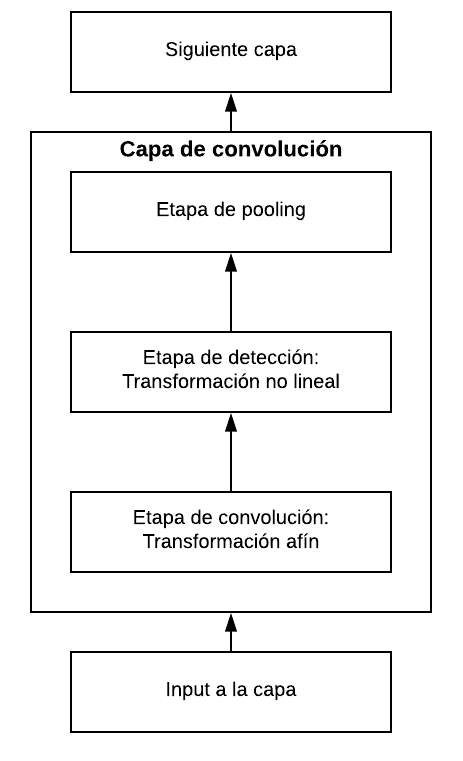
\includegraphics[scale=.8]{img/cap7_CNN.png}
\end{figure}

\textbf{Max pooling} retorna el valor m\'aximo de un output en una vecindad rectangular. Las operaciones de pooling permiten que la red sea invariante a peque{\~{n}}as transformaciones en el input. Pooling tambi\'en es escencial para procesar inputs de tama{\~{n}}o variable (por ejemplo im\'agenes de distinto tama{\~{n}}o).

Otras diferencias con respecto a la operaci\'on de convoluci\'on en el contexto de redes neuronales son, por ejemplo, el aplicar m\'ultiples convoluciones en paralelo, esto permite extraer distintos tipos de atributos en vez de 1 solo. Por otro lado, el \textbf{stride} hace referencia a cada cu\'antos pixeles se quieren convolucionar en cada direcci\'on en el output. En la figura se muestra el ejemplo de una convoluci\'on con stride. Esta operaci\'on permite reducir nuevamente el costo computacional. Esto tambi\'en implica que el output disminuye su tama{\~{n}}o en cada capa. El uso de \textit{padding} puede revertir esto. \textbf{Padding} se refiere a agrandar el input con ceros para hacerlo m\'as amplio. Una convoluci\'on en la que no se usa \textbf{zero-padding} se conoce como \textbf{valid}. Una convoluci\'on que mantiene el tama{\~{n}}o desde el input al output se conoce como \textbf{same} (ver figura). En la pr\'actica, las capas de una red convolucional usan operaciones entre una convoluci\'on valid y same.

\begin{figure}[H]
\captionsetup{font=small,labelfont=small}
\caption{Convoluci\'on con un stride igual a 2}
\centering
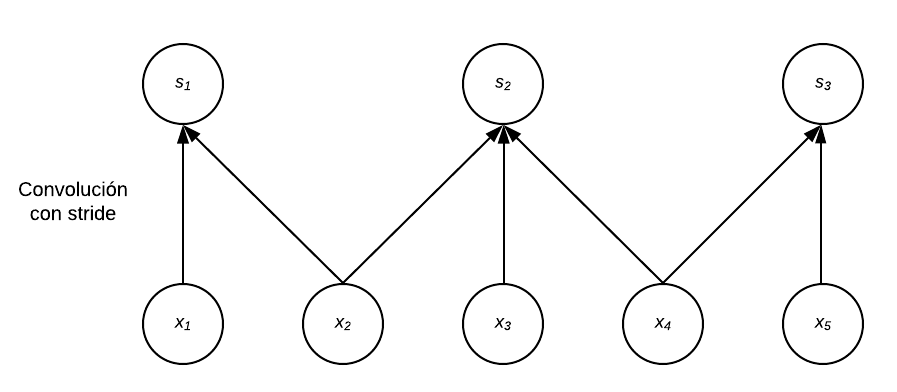
\includegraphics[scale=.8]{img/cap7_stride.png}
\end{figure}

\begin{figure}[H]
\captionsetup{font=small,labelfont=small}
\caption{Efecto de no usar zero-padding en una red convolucional (Arriba) y efecto de usar zero padding en una red convolucional (Abajo) en cuanto al tama{\~{n}}o de la red}
\centering
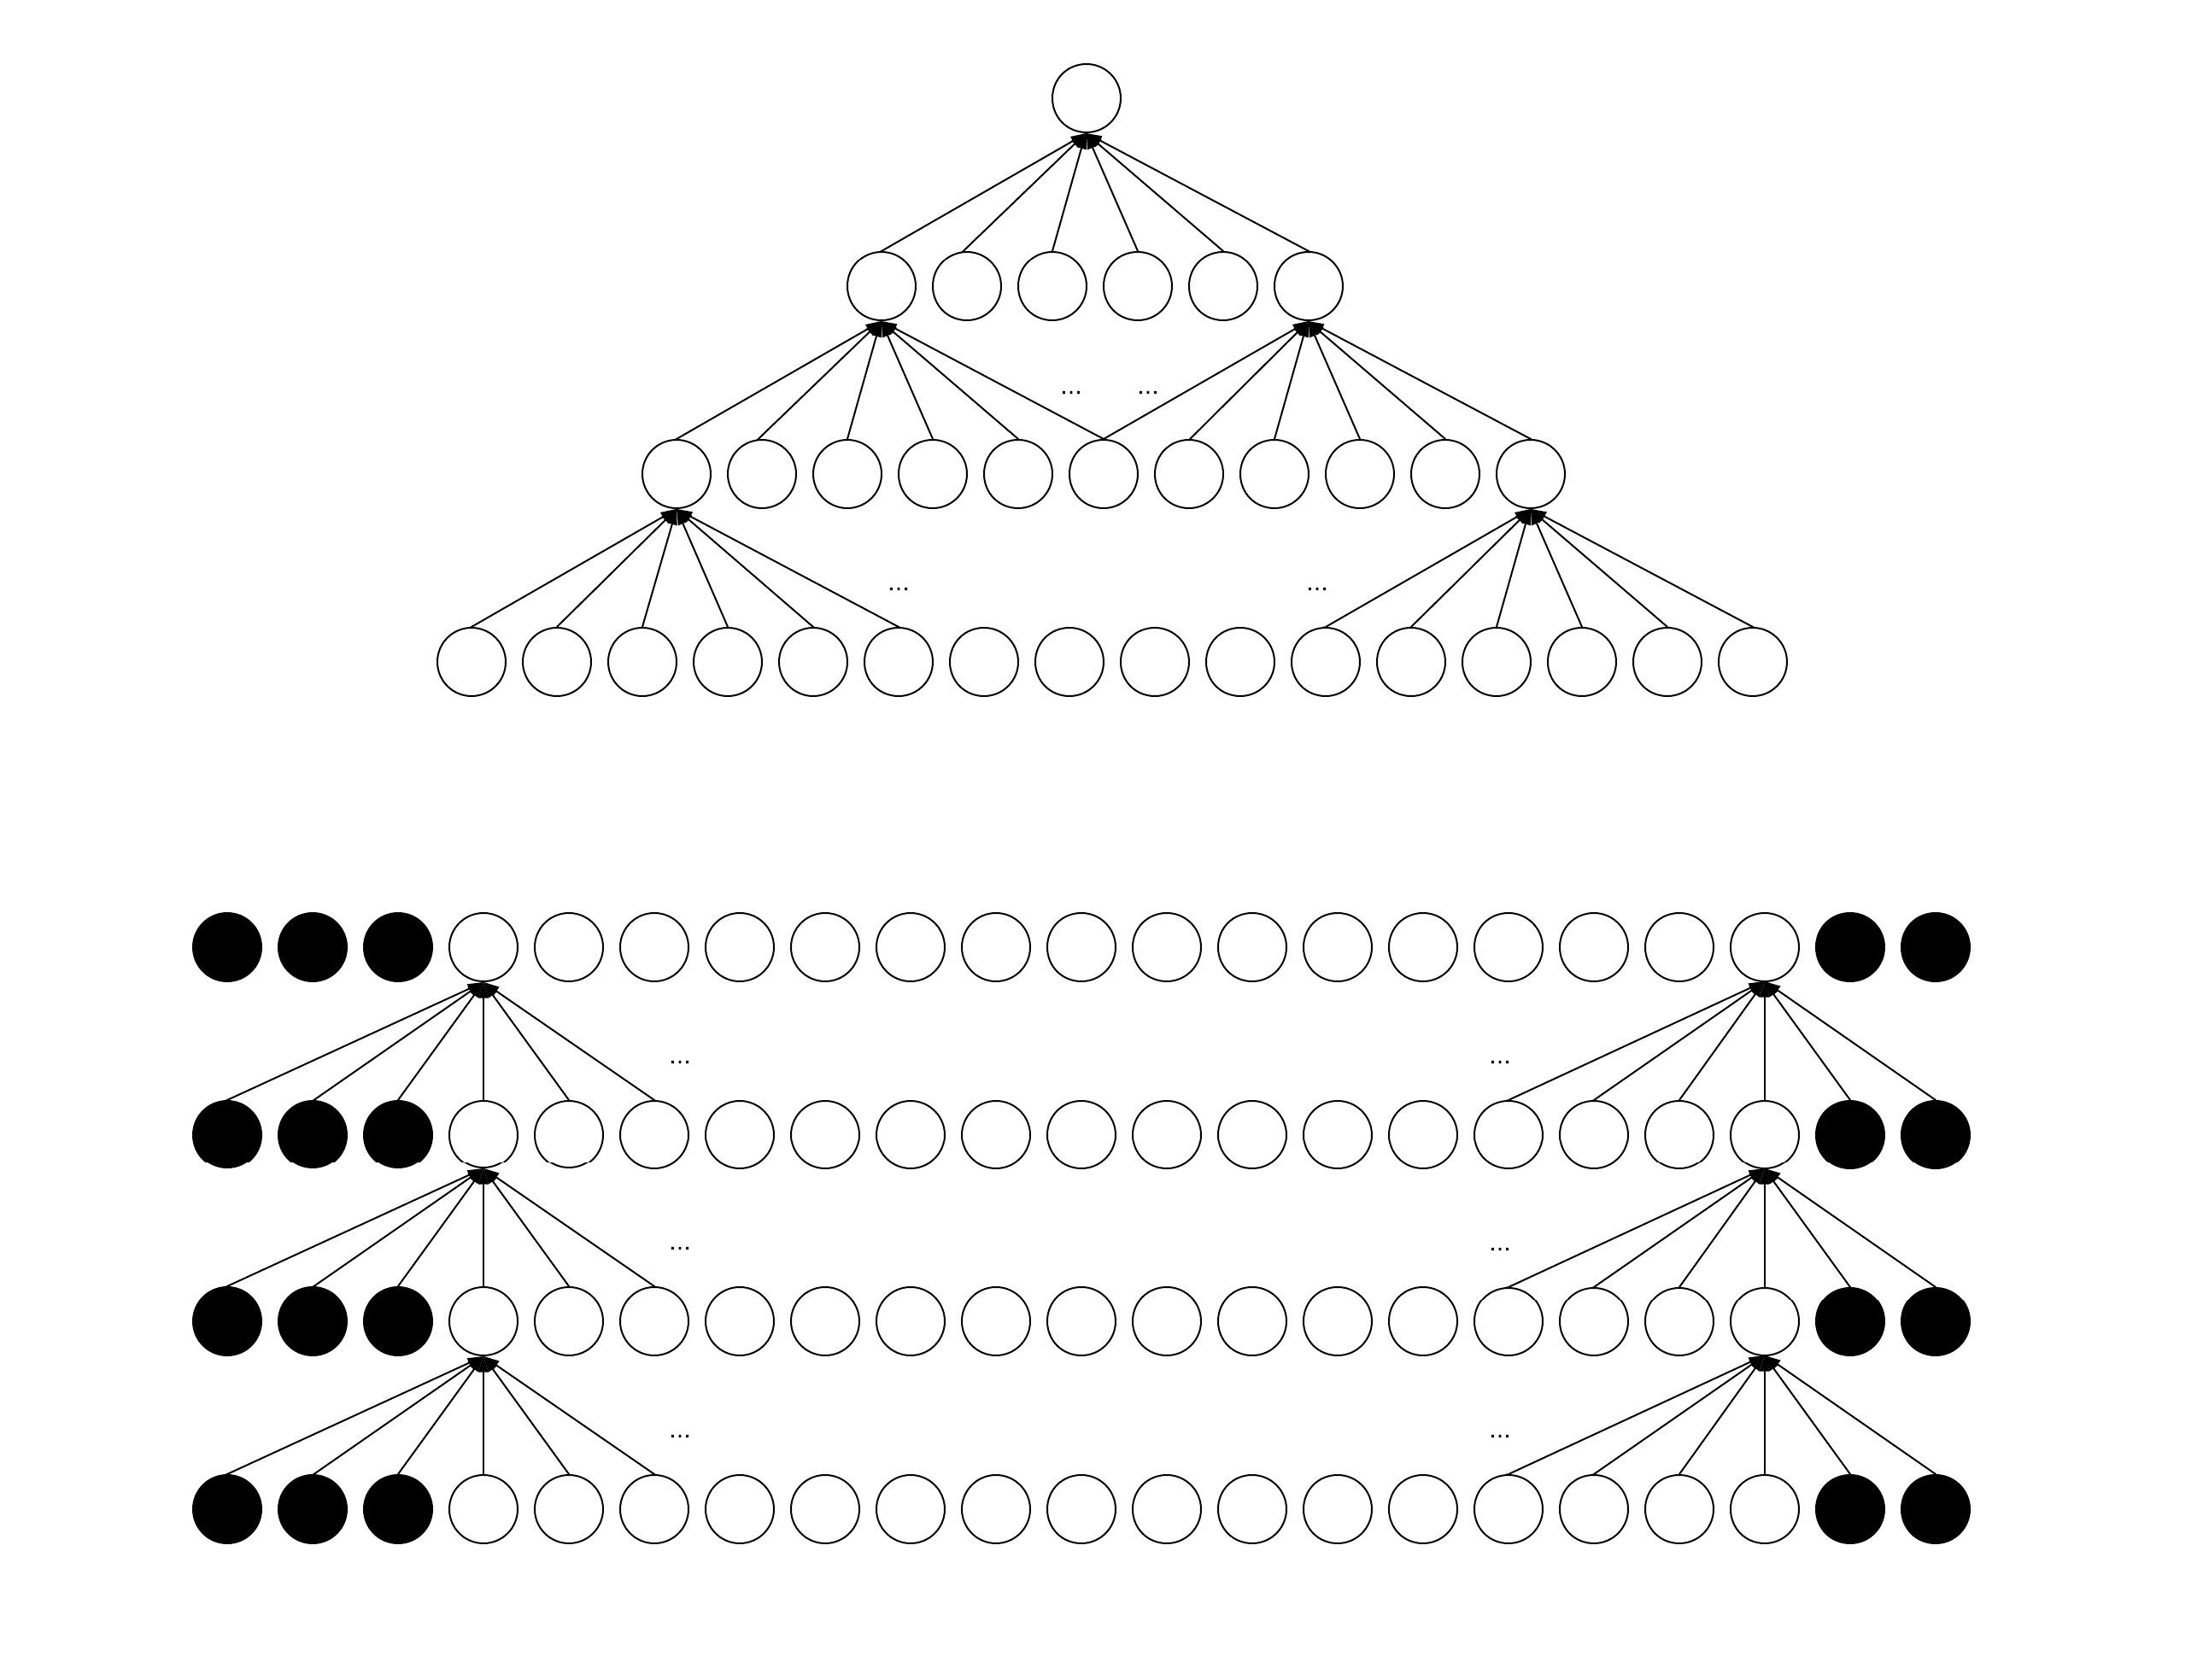
\includegraphics[scale=.15]{img/cap7_padding.png}
\end{figure}

\subsubsection{Redes neuronales recurrentes}

Las \textbf{redes neuronales recurrentes} o \textbf{RNNs} son una familia modelos de redes neuronales especializados para procesar datos secuenciales, $\bm{x}^{(1)},...,\bm{x}^{(\tau)}$. Las RNNs tambi\'en comparten par\'ametros, pero en una forma muy distinta que las CNNs. En una RNN, cada miembro del output en una etapa es una funci\'on de cada miembro del output de la etapa anterior.

Se denota por $\bm{h}^{(t)}$ al estado de un sistema din\'amico que involucra una recurrencia conducido por un input externo $\bm{x}^{(t)}$:

\begin{equation}
\bm{h}^{(t)} = f(\bm{h}^{(t-1)}; \bm{x}^{(t)}, \bm{\theta})
\end{equation}

La figura siguiente muestra una red recurrente que procesa un input $\bm{x}$ incorpor\'andolo al estado $\bm{h}$ que es traspasado a trav\'es del tiempo.

\begin{figure}[H]
\captionsetup{font=small,labelfont=small}
\caption{Ejemplo de una red recurrente sin output}
\centering
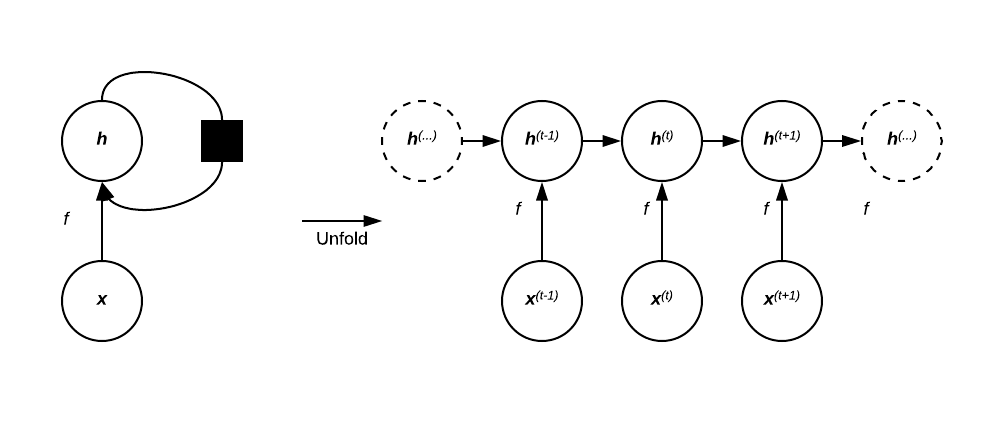
\includegraphics[scale=.5]{img/cap7_RNN1.png}
\end{figure}

Las redes recurrentes se pueden construir de muchas formas distintas. Al igual que una red neuronal puede representar casi cualquier funci\'on, una red recurrente modela cualquier funci\'on que involucre una recurrencia. Se puede representar el estado de una red recurrente luego de $t$ pasos mediante una funci\'on $g^{(t)}$:

\begin{equation}
\bm{h}^{(t)} = g^{(t)}(\bm{x}^{(t)},\bm{x}^{(t-1)},...,\bm{x}^{(1)}) =  f(\bm{h}^{(t-1)}; \bm{x}^{(t)}, \bm{\theta})
\end{equation}

Existen varios tipos de RNNs que se han dise{\~{n}}ado para distintos fines. Algunos ejemplos de estas son:

\begin{itemize}
  \item Redes recurrentes que producen un output en cada instante de tiempo y tienen conexiones entre todas las unidades escondidas
  \item Redes recurrentes que producen un output en cada instante de tiempo y tienen conexiones entre el output a la unidad escondida del siguiente instante
  \item Redes recurrentes con conexiones entre las unidad escondidas, que procesan una secuencia entera antes de producir el output
\end{itemize}

La figura muestra un ejemplo de la arquitectura para el primer caso.

\begin{figure}[H]
\captionsetup{font=small,labelfont=small}
\caption{Ejemplo de una red recurrente que produce un output en cada instante de tiempo, y que comparte el estado a trav\'es del tiempo}
\centering
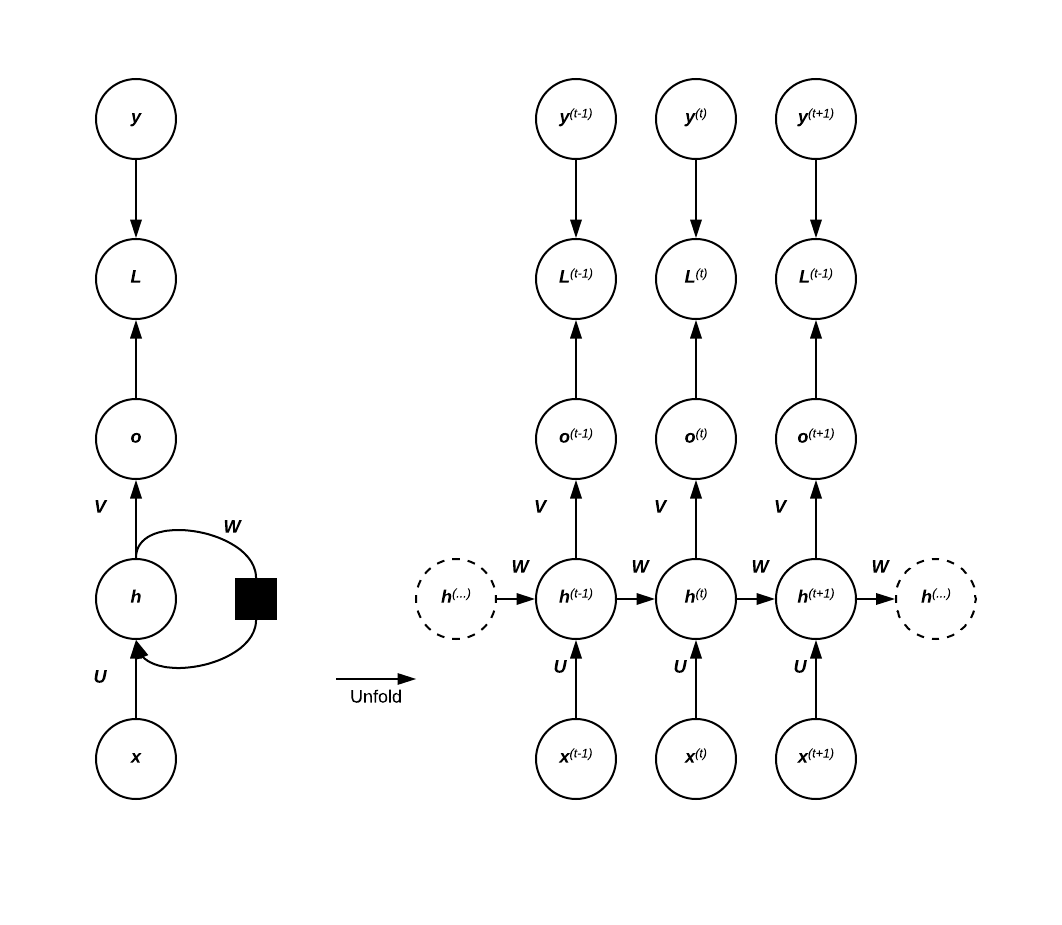
\includegraphics[scale=.5]{img/cap7_RNN2.png}
\end{figure}

Esta red presentada puede ser usada para producir palabras en cada instante, y as\'i producir oraciones que hagan sentido en una conversaci\'on. Como ejemplo de entrenamiento de una red con esta arquitectura, en donde en la \'ultima capa se decide mediante una funci\'on softmax la palabra m\'as probable que deba seguir a la palabra anterior, se tienen las ecuaciones de \textit{forward propagation} para cada instante de tiempo:

\begin{equation}
\begin{array}{l}
\bm{a}^{(t)} = \bm{b} + \bm{W}\bm{h}^{(t-1)}+\bm{U}\bm{x}^{(t-1)} \\
\bm{h}^{(t)} = \textrm{tanh}(\bm{a}^{(t)}) \\
\bm{o}^{(t)} = \bm{c} + \bm{V}\bm{h}^{(t)} \\
\hat{\bm{y}}^{(t)} = \textrm{softmax}(\bm{o}^{(t)})
\end{array}
\end{equation}

El algoritmo aplicado para obtener el gradiente en este tipo de arquitectura se conoce como \textbf{back-propagation through time}, y consiste en aplicar el algoritmo de \textit{back-propagation} generalizado para el grafo computacional \textit{unfolded} de la red, como los mostrados en las figuras de redes recurrentes.

Las redes recurrentes sufren de no poder recordar largas dependencias a trav\'es del tiempo, debido a que las recurrencias implican multiplicar una matriz de pesos m\'ultiples veces a trav\'es de la red, provocando superficies planas o muy empinadas que resultan en que los algoritmos de aprendizaje por gradiente tengan problemas de \textbf{vanishing gradients} o \textbf{exploding gradients}, respectivamente. Arquitecturas que han logrado superar esto son las que incluyen compuertas (funciones sigmoidales) que deciden autom\'aticamente qu\'e olvidar y qu\'e seguir propagando a trav\'es de la red. Estos son los modelos de \textbf{gated recurrent units} (\textbf{GRUs}) y \textbf{long-short term memory network} (\textbf{LSTM}).

\subsubsection{Autoencoders}

Un \textbf{autoencoder} es una red neuronal que busca replicar el input hacia el output, osea, se busca que la información que entra a la red sea lo más parecida posible a la de salida, para lo cual cuenta con una capa interna $\bm{h} = f(\bm{x})$ que codifica el input (genera una representaci\'on de este) llamada \textbf{encoder} y una funci\'on que produce la reconstrucci\'on $\bm{r} = g(\bm{h})$, el \textbf{decoder}. Un \textit{autoencoder} buscar\'a aprender los \textit{encoder} y \textit{decoder} tales que $g(f(\bm{x})) = \bm{x}$ para todo $\bm{x}$. Como el modelo est\'a forzado a aprender los atributos m\'as importantes para que pueda efectivamente reproducir el input en su output, este aprender\'a en general propiedades \'utiles de los datos de entrenamiento. Los \textit{autoencoders} modernos modelan mappings estoc\'asticos $p_{\textrm{encoder}}(\bm{h}|\bm{x})$ y $p_{\textrm{decoder}}(\bm{x}|\bm{h})$, en vez de funciones determin\'isticas. En la figura se muestra la arquitectura de un \textit{autoencoder}.

\begin{figure}[H]
\captionsetup{font=small,labelfont=small}
\caption{Estructura de un \textit{autoencoder} t\'ipico}
\centering
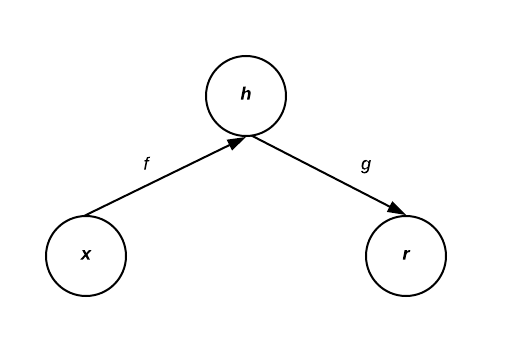
\includegraphics[scale=.8]{img/cap7_autoencoder.png}
\end{figure}

Una manera de obtener atributos \'utiles de $\bm{x}$ es forzando a que el \textit{encoder} tenga una dimensionalidad menor que el input. Este tipo de \textit{autoencoders} se denominan \textbf{undercomplete}. El aprendizaje se describe mediante la optimizaci\'on de la funci\'on de p\'erdida, $L(\bm{x}, g(f(\bm{x})))$. Cuando el \textit{decoder} es lineal y la funci\'on de p\'erdida es el error cuadr\'atico medio, un \textit{undercomplete autoencoder} aprende a generar el mismo subespacio que el algoritmo \textbf{principal component analysis} (\textbf{PCA}), es decir, el \textit{autoencoder} que fue entrenado para reproducir los datos de entrenamiento mediante una reducci\'on de dimensionalidad y una reconstrucci\'on aprendi\'o como efecto colateral el subespacio principal. Es as\'i como entonces, \textit{autoencoders} con \textit{encoders} y \textit{decoders} no lineales pueden aprender representaciones no lineales m\'as poderosas que PCA.

Un \textit{autoencoder} con dimensi\'on de su \textit{encoder} igual a la del input se conoce como \textbf{overcomplete}. Estos \textit{autoencoders}, al igual que los \textit{undercomplete}, pueden fallar en aprender una representaci\'on \'util del input si tienen mucha capacidad, por lo que ser\'a importante tambi\'en regularizar estas redes neuronales.

Otras aplicaciones de los autoencoders, aparte de aprender una reducci\'on de dimensionalidad, es aprender representaciones \'utiles que sirvan para un posterior modelo de redes neuronales (o, m\'as general, de aprendizaje de m\'aquinas). Por ejemplo, en vez de usar \textbf{one-hot-vectors} para representar palabras (en donde se tiene un vector del largo de cierto vocabulario compuesto por ceros excepto para la palabra que se quiere representar, indicando un valor de 1 en esa posici\'on), se pueden usar \textbf{embeddings}, que son representaciones del input a un espacio de valores reales. A diferencia de los \textit{one-hot-vectors}, en un \textit{embedding} la distancia entre las representaciones del texto s\'i tiene un significado, y este tipo de representaciones podr\'ia entregar mejores resultados en la tarea en que se est\'e usando.

\subsubsection{Redes generativas adversariales}

Una \textbf{red generativa adversarial} (o \textbf{GAN}) se basa en un escenario de teor\'ia de juegos, en donde una \textbf{red generadora} debe competir con un adversario. La red generadora produce muestras $\bm{x} = g(\bm{z};\bm{\theta}^{(g)})$, mientras que una \textbf{red discriminadora} trata de distinguir entre muestras obtenidas de los datos de entrenamiento y muestras generadas por la red generadora. El discriminador retorna una probabilidad, $d(\bm{x};\bm{\theta}^{(d)})$, indicando la probabilidad de que $\bm{x}$ sea un dato real y no uno simulado.

Para formular el aprendizaje, se describe un juego de suma cero en donde una funci\'on $v(\bm{\theta}^{(g)},\bm{\theta}^{(d)})$ determina el pago del discriminador, y el generador recibe $-v(\bm{\theta}^{(g)},\bm{\theta}^{(d)})$ como pago. As\'i, durante el entrenamiento cada jugador intenta maximizar su propio pago, para que en convergencia se tenga

\begin{equation}
g^{*} = \textrm{arg} \textrm{min}_{g} \textrm{max}_{d} v(g,d)
\end{equation}

Esto motiva a que el discriminador aprenda a clasificar correctamente entre muestras reales y falsas y, simulat\'aneamente, el generador intenta enga{\~{n}}ar al clasificador para que crea que las muestras generadas son reales. En convergencia, las muestras del generador son indistinguibles de los datos reales. Una motivaci\'on del uso de GANs es que cuando $\textrm{max}_{d} v(g,d)$ es convexa en $\bm{\theta}^{(g)}$, el procedimiento asegura la convergencia.

\begin{figure}[H]
\captionsetup{font=small,labelfont=small}
\caption{Im\'agenes generadas por una GAN entrenada con el set de datos LSUN. (Izquierda) Im\'agenes de dormitorios generadas por el modelo DCGAN (imagen de Radford et al., 2015). (Derecha) Im\'agenes de iglesias generadas por el modelo LAPGAN (imagen de Denton et al., 2015)}
\centering
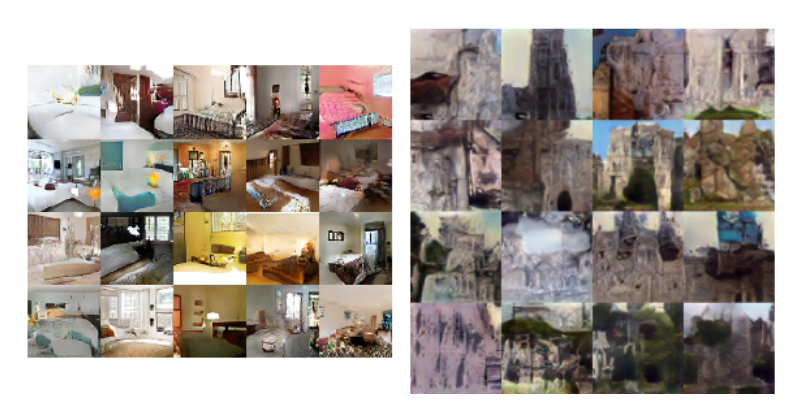
\includegraphics[scale=.75]{img/cap7_gans.PNG}
\end{figure}
